\documentclass{article}

\usepackage[%
    left=0.5in,%
    right=0.5in,%
    top=0.5in,%
    bottom=0.5in,%
]{geometry}%
\usepackage{minitoc}
\usepackage{multicol}
\usepackage{graphicx}
\usepackage{fixltx2e}
\usepackage{listings}
\usepackage{color}
\usepackage{hyperref}
    \hypersetup{ colorlinks = true, linkcolor = blue }
\usepackage{blindtext}
\definecolor{lightgray}{gray}{0.9}
\graphicspath{ {./} }

\newcommand{\inlinecode}[2]{\colorbox{lightgray}{\lstinline
[language=#1]$#2$}}
\newcommand{\worddef}[1]{\hyperref[sec:reference]{\textit{#1}}}

\begin{document}

\tableofcontents

\newpage

\section{Von Neumann Architecture}
\begin{flushleft}
A simple abstraction of a general purpose digital computer
\begin{itemize}
  \item All program instructions and data are stored in a \textbf{single memory unit}
  \item The CPU fetches instructions and executes them, in sequence, using the ALU
  \item The memory is \textbf{read-write} and random access, i.e. any location in memory can be accessed as easily/quickly \textbf{as any other}. Unlike, for example, tape storage
\end{itemize}
\end{flushleft}

\section{Memory hierarchy}

\subsection{Main Memory and Registers}
\begin{flushleft}
Main memory is \textbf{separate} from CPU.
\begin{itemize}
  \item Explicitly addressed by program instructions
  \item Contains all program code and almost all data
  \item Is \textbf{slow to access} compared to one ALU operation
\end{itemize}
Registers are built into CPU
\begin{itemize}
  \item \textbf{Explicitly named} by program instructions
  \item Contain just a few local (local) variables / parameters
  \item \textbf{Very fast to access but very limited}
\end{itemize}
\end{flushleft}

\subsection{Cache}
\begin{flushleft}
Cache is used to improve main memory performance
\begin{itemize}
  \item Built into CPU (like registers)
  \item \textbf{Not directly visible} to program code (unlike registers)
  \item Temporarily stores code/data \textbf{fetched from main memory}
  \item Limited size: only stores recently requested, used or anticipated code/data
  \item Faster to access than main memory \textbf{once loaded}
  \begin{itemize}
    \item Repeating code (e.g. loop) is faster than sequential code 
    \item Repeated data access is faster than one-off data access
  \end{itemize}
\end{itemize}
\end{flushleft}

\subsubsection{Cache levels}

\begin{itemize}
  \item Level 1 Instruction (L1-I) cache: program code being executed (a few kB)
  \item Level 1 Data (L1-D) cache: data from main memory being used right now (a few kB)
  \item Level 2 Unified (Instruction and Data) cache – (a few MB)
  \item (may be more levels)
\end{itemize}

\begin{multicols}{2}

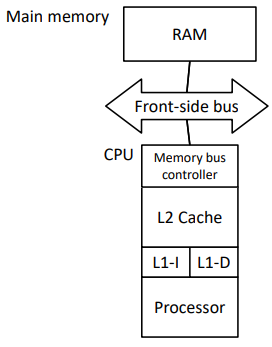
\includegraphics[scale=0.5]{cache_levels.png}

\end{multicols}

\pagebreak
\section*{Reference section} \label{sec:reference}
\begin{description}
	\item[placeholder] \hfill \\
\end{description}
\end{document}
